\documentclass[12pt,a4paper]{article}

% ============================================================
% PACKAGES
% ============================================================
\usepackage[a4paper,margin=1in]{geometry}
\usepackage{times}
\usepackage{setspace}
\usepackage{graphicx}
\usepackage{float}
\usepackage{booktabs}
\usepackage{array}
\usepackage{multirow}
\usepackage{longtable}
\usepackage{tabularx}
\usepackage{amsmath,amssymb}
\usepackage{algorithm}
\usepackage{algpseudocode}
\usepackage{xcolor}
\usepackage{listings}
\usepackage{tikz}
\usepackage{pgfplots}
\usepackage{caption}
\usepackage{subcaption}
\usepackage{hyperref}
\usepackage{enumitem}
\usepackage{fancyhdr}
\usepackage{titlesec}

\usetikzlibrary{
    shapes.geometric,
    arrows.meta,
    positioning,
    fit,
    calc,
    backgrounds
}

\pgfplotsset{compat=1.18}

% ============================================================
% HYPERLINKS
% ============================================================
\hypersetup{
    colorlinks=true,
    linkcolor=blue,
    citecolor=blue,
    urlcolor=blue,
    pdftitle={Intelligent Compiler for Detecting Errors in Medical Data Processing Programs Using GAN}
}

% ============================================================
% LINE SPACING
% ============================================================
\onehalfspacing
\setlength{\parskip}{0.2em}

% ============================================================
% HEADER / FOOTER
% ============================================================
\pagestyle{fancy}
\fancyhf{}
\fancyhead[L]{Compiler Design Lab (CSE3024)}
\fancyhead[R]{VIT-AP University}
\fancyfoot[C]{\thepage}
\setlength{\headheight}{14.5pt}

% ============================================================
% CODE STYLE
% ============================================================
\definecolor{codegreen}{rgb}{0,0.5,0}
\definecolor{codegray}{rgb}{0.5,0.5,0.5}
\definecolor{codepurple}{rgb}{0.58,0,0.82}

\lstdefinelanguage{MedScript}{
    morekeywords={input,const,func,let,if,else,while,return,true,false,int,float,bool,string,phi,range},
    morekeywords=[2]{kg,lb,gram,mg,ml,bpm,mmHg,degC,degF,metre,hour},
    morekeywords=[3]{print,export,present,anonymize,lb_to_kg,degF_to_degC,g_to_mg,abs,min,max},
    keywordstyle=\color{blue}\bfseries,
    keywordstyle=[2]\color{orange!80!black},
    keywordstyle=[3]\color{purple},
    sensitive=true,
    morecomment=[l]{//},
    morestring=[b]"
}

\lstset{
    language=C,
    basicstyle=\ttfamily\footnotesize,
    keywordstyle=\color{blue},
    commentstyle=\color{codegreen},
    stringstyle=\color{codepurple},
    numbers=left,
    numberstyle=\tiny\color{codegray},
    stepnumber=1,
    numbersep=8pt,
    frame=single,
    breaklines=true,
    showstringspaces=false,
    xleftmargin=1.6em,
    framexleftmargin=1.2em
}

% ============================================================
% TITLE FORMAT
% ============================================================
\titleformat{\section}
{\large\bfseries}
{\thesection.}{0.5em}{}

\titleformat{\subsection}
{\normalsize\bfseries}
{\thesubsection}{0.5em}{}

\captionsetup{font=small,labelfont=bf}
\newcommand{\code}[1]{\texttt{#1}}
\newcommand{\ie}{\textit{i.e.,}\xspace}
\providecommand{\xspace}{}

\newcommand{\NProg}{10{,}000}
\newcommand{\NFeat}{101}
\newcommand{\NTrain}{8{,}000}
\newcommand{\NTest}{2{,}000}
\newcommand{\MeanLoc}{38.7}
\newcommand{\TotalLoc}{386{,}953}
\newcommand{\NDouble}{1{,}398}
\newcommand{\DoubleShare}{15.5}
\newcommand{\RuleFirstAcc}{91.6}
\newcommand{\RulePrioAcc}{93.2}
\newcommand{\RuleFirstDouble}{65.7}
\newcommand{\RFAcc}{99.15}
\newcommand{\MLPAcc}{99.35}
\newcommand{\HGBAcc}{99.40}
\newcommand{\LRAcc}{99.20}
\newcommand{\RFMacro}{0.9915}
\newcommand{\RFDouble}{96.4}
\newcommand{\RuleLogicRecall}{68.5}
\newcommand{\RFLogicRecall}{97.0}
\newcommand{\MsPerKloc}{162}
\newcommand{\ScaleRSq}{0.981}
\newcommand{\ScaleSlope}{1.17}
\newcommand{\OptMean}{8.9}
\newcommand{\OptMax}{17.8}
\newcommand{\OptPrograms}{300}
\newcommand{\OptMismatch}{0}
\newcommand{\AugMinutes}{34}
\newcommand{\HeldoutNN}{7.4}


\begin{document}

% ============================================================
% PAGE 1 -- TITLE PAGE
% ============================================================
\begin{titlepage}
\begin{center}

\vspace*{0.2cm}


\includegraphics[width=9cm,trim=0 185 0 185,clip]{vit-ap-university-logo.png}

\vspace{0.2cm}

{\large
Amaravati, Andhra Pradesh, India
}

\vspace{0.7cm}

{\Large\bfseries
COMPILER DESIGN LAB REPORT
}

\vspace{0.3cm}

{\large
\textbf{Subject Name: Compiler Design Lab}
}

\vspace{0.1cm}

{\large
\textbf{Course Code: CSE3024}
}

\vspace{0.8cm}

{\LARGE\bfseries
Intelligent Compiler for Detecting Errors in\\
Medical Data Processing Programs Using GAN
}

\vspace{0.6cm}

\begin{tabular}{rl}
\textbf{Compiler Design Component:} & Parsing \& Semantic Analysis\\[0.15cm]
\textbf{Machine Learning Component:} & Error Classification\\[0.15cm]
\textbf{Application Domain:} & Healthcare
\end{tabular}

\vspace{1.0cm}

\textbf{Submitted by}

\vspace{0.4cm}

\begin{tabular}{ll}
\textbf{Swarnim Bandekar} & \textbf{Regd. No.:} 24BCB7157 \\[0.4cm]
\textbf{Lithin CG} & \textbf{Regd. No.:} 24BCB7016 \\
\end{tabular}

\vspace{1.0cm}

\textbf{Under the Guidance of}

\vspace{0.3cm}

\textbf{Dr. Prakash Kumar Sarangi}

\vspace{1.0cm}

{\large
School of Computer Science and Engineering (SCOPE)\\
VIT-AP University\\
Amaravati, Andhra Pradesh, India
}

\vspace{0.4cm}

{\large
Academic Year 2026--2027
}

\end{center}
\end{titlepage}

% ============================================================
% ABSTRACT
% ============================================================
\section*{Abstract}

Programs that process medical data can contain mistakes that a general-purpose compiler never reports: a dose added to a
body weight, a temperature threshold typed ten times too large, a laboratory value that may be missing but is used
unguarded, or a patient name that reaches a log file. This report describes a compiler front end built to catch such
errors, and a learned classifier that sits on top of it and names the root-cause family of each defective program.

The front end is written for MedScript, a small domain-specific language that we designed with units of measure in its types,
declared physiological ranges, protected-health-information tagging and optional values. It consists of a hand-written lexer,
a recursive-descent parser with error recovery, and a semantic analyser that checks types and units, interval-based range
plausibility, taint flow of patient identifiers, presence of optional values, definite assignment and division by zero. A
three-address-code generator, a six-pass optimiser and a virtual machine complete the pipeline. On a synthetic corpus of
\NProg{} programs in ten classes (valid, plus nine error families injected by 46 mutation operators), the learned
classifiers, which use features computed by the compiler, reach \RFAcc\% accuracy, against \RuleFirstAcc\% for taking the family of the first
diagnostic. They also catch faults the compiler cannot see, such as an inverted fever rule, which a rule-based reading of its diagnostics misses.

A conditional generative adversarial network was trained on the feature vectors to supply synthetic examples of rare error classes.
In ten-seed experiments with 5 to 100 real examples per class, it did not help: Gaussian jitter and SMOTE performed better, and only
about 4\% of the GAN's samples were recognisable as the requested class. A GAN discriminator trained on valid programs only did
detect the compiler-invisible faults well (AUROC 0.98), although its results on other fault families are largely explained by the diagnostic features.
The compiler processes about \MsPerKloc{} ms per thousand lines, and its optimiser preserved program behaviour in all tested cases.
The corpus is synthetic and the results should be read accordingly.

\vspace{0.4em}
\textbf{Keywords:}
Compiler Design, Semantic Analysis, Parsing, Units of Measure, Error Classification, Generative Adversarial Network,
Healthcare Software.

\newpage

% ============================================================
% INTRODUCTION
% ============================================================
\section{Introduction}

Programs that handle medical data are usually small and unglamorous: a script that flags abnormal vital signs, a
routine that turns a body weight into a drug dose, a nightly job that exports records to a research registry. A
mistake in any of them can still reach a patient. The Therac-25 overdoses were traced to defects in control
software \cite{leveson1993}, and the Mars Climate Orbiter was lost because one team produced impulse data in
pound-force seconds while the consuming software expected newton seconds \cite{mco1999}. In compiler terms the second
failure is a plain type error that the type system could not see, because both quantities were just \code{double}.

Clinical code has the same weak spot. A dose in milligrams added to a weight in kilograms, a fever threshold typed as
\code{380} instead of \code{38.0}, a lab value that may be missing but is used as if it were always present, or a
patient name written to a log: all of these are syntactically fine and pass through a general-purpose compiler without
a word. The knowledge needed to catch them (units, physiological ranges, privacy rules) lives in the programmer's
head, not in the language.

This project builds a compiler front end that does know about that domain, and then asks a machine-learning question
on top of it: can a learned model tell us what kind of mistake a program contains, even when the compiler's own
diagnostics are incomplete or misleading? The GAN comes in for a practical reason. Labelled examples of faulty
medical programs are scarce and hard to share, so a conditional GAN that learns compiler-derived feature vectors per
error class could supply extra training records without exposing any source code. Whether that actually helps is an
empirical question, and we report what we measured, including where it did not help.

\subsection{Motivation and Problem Statement}

Three observations drove the work. First, mainstream compilers check that an expression is a number, not that it is
a mass; units-of-measure systems exist \cite{kennedy1994} but not in the languages clinical scripts are written in.
Second, rule-based diagnostics are precise but narrow. Nothing in the grammar or the type system is violated by
\code{if (temp < 38.0 degC)} followed by an alert called ``fever'', and when several faults coexist the first message
is often not the root cause. Third, learned bug finders need large corpora \cite{allamanis2018,pradel2018}, which a
regulated domain does not have.

The problem we address is therefore: given the source of a medical data-processing program, (i) detect lexical,
syntactic, type, unit, range, privacy and missing-value errors with a purpose-built front end, and (ii) assign each
defective program to its root-cause error family with a classifier trained on compiler-derived features, using a GAN
to make up for the shortage of labelled faulty programs.

\subsection{Objectives and Contributions}

\begin{itemize}
    \item \textbf{MedScript and its compiler.} A small language with units in its types, PHI tagging, optional values
    and declared physiological ranges, plus a Python implementation (about 1{,}900 lines for the compiler, 4{,}900
    with corpus tools, learning code and tests) of lexer, parser with error recovery, semantic analyser, three-address
    code, a six-pass optimiser and a virtual machine. 38 unit tests accompany it.
    \item \textbf{Clinical safety rules as semantic checks.} Unit checking with exponent vectors, interval reasoning over
    declared ranges, taint tracking from \code{phi} inputs to output sinks, and flow-sensitive handling of optional values.
    \item \textbf{A fault-injection corpus} of \NProg{} programs in ten classes, produced by 46 mutation operators, with
    \DoubleShare\% of the faulty programs containing two faults.
    \item \textbf{Rule-based versus learned classification.} The learned classifiers reach \RFAcc\% accuracy against
    \RuleFirstAcc\% for reading the first diagnostic, and they catch faults the compiler cannot see.
    \item \textbf{A measured evaluation of GAN augmentation} over ten seeds and five levels of data scarcity, against
    simple resampling, plus a GAN-based anomaly detector. The GAN did not help classification, and we show why.
\end{itemize}

Section~2 reviews related work, Section~3 describes the language, compiler and learning components, Section~4 the
corpus and protocol, Section~5 the results, and Section~6 concludes.

% ============================================================
% RELATED WORK
% ============================================================
\section{Related Work}

\paragraph{Compiler front ends.} Lexing, parsing and semantic analysis follow Aho et al.~\cite{aho2006} and Cooper and
Torczon~\cite{cooper2007}. We use two ideas from that literature. One is error recovery: our recursive-descent parser
inserts a missing closing token where it can and otherwise skips to the next statement boundary, a mix of the local
repair and panic-mode schemes described by Burke and Fisher~\cite{burke1987} and Grune and Jacobs~\cite{grune2008}. The
other is phase gating: semantic analysis only runs on input the parser accepted. Section~5 shows this has a measurable
effect on programs with several faults. The flow-sensitive parts of our analyser are instances of the data-flow
framework of Nielson et al.~\cite{nielson1999}.

\paragraph{Units and information flow.} Kennedy's dimension types~\cite{kennedy1994} give each numeric type a unit
written as a product of base units with integer powers. Multiplication adds exponents, division subtracts them, and
addition requires them to match. That single rule would have caught both the Mars Climate Orbiter error and the
dose-plus-weight mistake, and it is what we use. Taint analysis tracks data from sources to sinks; TaintDroid
\cite{enck2010} does it at run time on smartphones. We use a static variant in which \code{phi} inputs are tainted and
only \code{anonymize()} clears the taint, motivated by the HIPAA Privacy Rule~\cite{hipaa}.

\paragraph{Learning for program defects.} Allamanis et al.~\cite{allamanis2018} survey statistical models of code.
DeepFix~\cite{gupta2017} repairs syntax and type errors in student C programs, and DeepBugs~\cite{pradel2018} learns
name-based detectors for bugs such as swapped arguments, close in spirit to our inverted-comparison faults. These
systems learn from tokens or graphs of general-purpose code. We go lighter: the model sees what the compiler already
computed (diagnostic counts, structural statistics, a few clinical-rule patterns), so it stays small and its inputs
stay readable.

\paragraph{GANs and imbalanced data.} A GAN trains a generator against a discriminator~\cite{goodfellow2014}; the
conditional version feeds a class label to both~\cite{mirza2014}. Training is unstable, which led to label
smoothing~\cite{salimans2016} and the Wasserstein objective with gradient penalty~\cite{arjovsky2017,gulrajani2017}.
medGAN~\cite{choi2017} and CTGAN~\cite{xu2019} generate synthetic patient records and tabular data. The classical
answers to class imbalance are random oversampling and SMOTE~\cite{chawla2002}. A GAN trained on normal data can also
score anomalies, as in AnoGAN~\cite{schlegl2017}; we compare a lighter version of that idea with Isolation
Forest~\cite{liu2008} and the one-class SVM~\cite{scholkopf2001}.

\paragraph{Gap.} None of these systems combines a front end with clinical semantics, a learned classifier on top of it
that reasons about root cause, and a test of GAN augmentation against cheap resampling on the same task. This project
tries that combination at lab scale, with a purpose-built DSL and a synthetic corpus.

% ============================================================
% PROPOSED METHODOLOGY
% ============================================================
\section{Proposed Methodology}

\subsection{System Overview}

The system has two halves (Figure~\ref{fig:arch}). The compiler half is a conventional pipeline (scanner, parser,
semantic analyser, intermediate-code generator, optimiser) for a language called MedScript, and every phase reports
diagnostics with a stable code, a position and a message. The learning half condenses the tokens, syntax tree and
diagnostics into a fixed-length feature vector, and a classifier maps it to one of ten classes: \emph{valid} or one of
nine error families. A conditional GAN trained on the labelled vectors supplies extra records of rare classes at
training time only. What gets deployed is the compiler plus a random forest.

\begin{figure}[!htbp]
\centering
\resizebox{0.92\textwidth}{!}{%
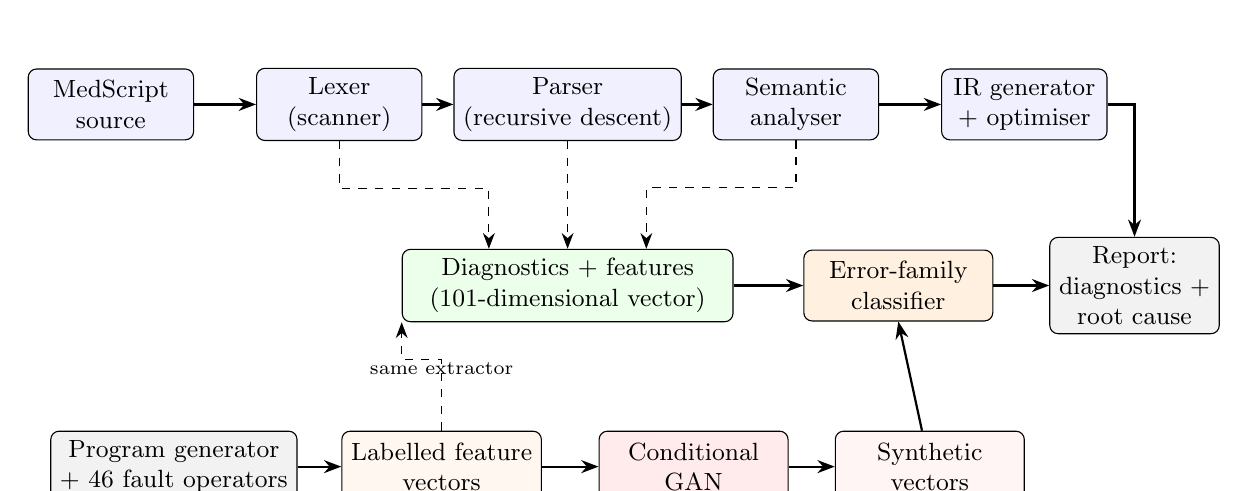
\begin{tikzpicture}[
  box/.style={rectangle,rounded corners=3pt,draw,minimum height=0.9cm,minimum width=2.1cm,align=center,font=\small,fill=blue!6},
  ml/.style={rectangle,rounded corners=3pt,draw,minimum height=0.9cm,minimum width=2.4cm,align=center,font=\small,fill=orange!12},
  gan/.style={rectangle,rounded corners=3pt,draw,minimum height=0.9cm,minimum width=2.4cm,align=center,font=\small,fill=red!8},
  arr/.style={-{Stealth[length=2.2mm]},thick},
  dsh/.style={-{Stealth[length=2mm]},dashed}
]
\node[box] (src) at (0,0) {MedScript\\source};
\node[box] (lex) at (2.9,0) {Lexer\\(scanner)};
\node[box] (par) at (5.8,0) {Parser\\(recursive descent)};
\node[box] (sem) at (8.7,0) {Semantic\\analyser};
\node[box] (ir)  at (11.6,0) {IR generator\\+ optimiser};
\draw[arr] (src) -- (lex);
\draw[arr] (lex) -- (par);
\draw[arr] (par) -- (sem);
\draw[arr] (sem) -- (ir);

\node[box,fill=green!8,minimum width=4.2cm] (diag) at (5.8,-2.3) {Diagnostics + features\\(101-dimensional vector)};
\draw[dsh] (lex.south) -- ++(0,-0.6) -| ($(diag.north)+(-1.0,0)$);
\draw[dsh] (par.south) -- (diag.north);
\draw[dsh] (sem.south) -- ++(0,-0.6) -| ($(diag.north)+(1.0,0)$);

\node[ml] (clf) at (10.0,-2.3) {Error-family\\classifier};
\draw[arr] (diag) -- (clf);
\node[box,fill=gray!10] (rep) at (13.0,-2.3) {Report:\\diagnostics +\\root cause};
\draw[arr] (clf) -- (rep);
\draw[arr] (ir) -- (13.0,0) -- (rep.north);

\node[box,fill=gray!10] (gen) at (0.8,-4.6) {Program generator\\+ 46 fault operators};
\node[ml,fill=orange!6] (corp) at (4.2,-4.6) {Labelled feature\\vectors};
\node[gan] (cg) at (7.4,-4.6) {Conditional\\GAN};
\node[gan,fill=red!4] (syn) at (10.4,-4.6) {Synthetic\\vectors};
\draw[arr] (gen) -- (corp);
\draw[arr] (corp) -- (cg);
\draw[arr] (cg) -- (syn);
\draw[arr] (syn) -- (clf.south);
\draw[dsh] (corp.north) -- ++(0,0.9) -| (diag.south west);
\node[font=\scriptsize,align=center] at (4.2,-3.35) {same extractor};
\end{tikzpicture}}
\caption{System architecture. Solid arrows are data flow, dashed arrows are diagnostics and features collected from
the compiler phases. The GAN branch (bottom) is only used to enlarge the training set.}
\label{fig:arch}
\end{figure}

\subsection{The MedScript Language}

MedScript is small on purpose: enough to write the programs a clinical-informatics student would write, and enough
machinery to make the domain checks meaningful.

\begin{itemize}
    \item \textbf{Units are part of the type.} A numeric type is \code{int}, \code{float}, or a float with a unit such
    as \code{kg}, \code{mg/kg} or \code{kg/metre\textasciicircum 2}. Literals carry units: \code{38.0 degC}. The
    vocabulary has eleven units (\code{kg}, \code{lb}, \code{gram}, \code{mg}, \code{ml}, \code{hour}, \code{bpm},
    \code{mmHg}, \code{degC}, \code{degF}, \code{metre}), each with a plausible literal range such as 20 to 45 for \code{degC}.
    \item \textbf{Inputs carry metadata.} \code{input weight: kg range(2, 300);} declares a read-only patient value with
    a physiological range, and \code{phi} marks protected health information.
    \item \textbf{Optional values.} A trailing \code{?} means the value may be missing and must be tested with
    \code{present(x)} before use.
    \item \textbf{Two sinks}, \code{print} and \code{export}, which reject PHI unless it went through \code{anonymize}.
    \item \textbf{Ordinary control flow}: \code{if}/\code{else}, \code{while}, typed functions and \code{let} bindings.
\end{itemize}

Listing~\ref{lst:ok} shows a program the compiler accepts: a capped weight-based dose, a BMI, a fever alert, a sepsis
screen, a guarded check on a possibly missing lab value, and an anonymised export.

\begin{lstlisting}[language=MedScript,caption={A valid MedScript program (\texttt{examples/triage\_ok.med}).},label={lst:ok}]
input patient_name: string phi;
input weight: kg range(2, 300);
input temp: degC range(30, 43);
input hr: bpm range(20, 250);
input lactate: mg? range(0, 400);
const MAX_DOSE: mg = 1000 mg;

func dose_for(w: kg, rate: mg/kg) -> mg {
    let d: mg = rate * w;
    if (d > MAX_DOSE) { return MAX_DOSE; }
    return d;
}
let dose: mg = dose_for(weight, 15 mg/kg);
let fever = false;
if (temp > 38.0 degC) { fever = true; print("fever alert"); }
if (hr > 100 bpm && fever) { print("sepsis screen"); }
if (present(lactate)) {
    if (lactate > 200 mg) { print("high lactate"); }
}
export(anonymize(patient_name));
print(dose);
\end{lstlisting}

\subsection{Lexical and Syntax Analysis}

The scanner is a hand-written, single-pass, longest-match recogniser for identifiers, 16 keywords, 11 unit words,
numbers, strings, operators and \code{//} comments. A numeric lexeme is collected as the longest run of letters, digits
and dots and only then checked against $[0\text{-}9]^+(.[0\text{-}9]^+)?$, so \code{3.4.5} is reported as one bad
number instead of a number plus junk. The three lexical errors (illegal character, malformed number, unterminated
string; \code{LEX001} to \code{LEX003}) are all recoverable, so later phases still run. That matters for
classification: a lexical error does not hide semantic faults, but a syntax error does.

The grammar is LL(1) except in two places. A statement starting with an identifier needs one extra token to choose
between assignment and call, and after a number and a unit, a \code{/} belongs to the unit only if another unit follows.
Expressions use precedence climbing over six levels. Error recovery combines two mechanisms. A missing \code{;},
\code{)} or \code{\}} is reported as \code{SYN001} at the end of the previous token, where a programmer expects to see
it, and parsing continues as if the token were there. When an expression cannot start (\code{SYN002}), the parser skips
to the next semicolon or statement keyword. At most one diagnostic is issued per position, which removes most duplicate
cascades. If any syntax error was reported, semantic analysis is skipped.

\subsection{Semantic Analysis}

The analyser walks the tree once with a stack of scopes and a small flow state. This is where the clinical knowledge
lives. Functions are collected in a first pass, so calls can come before definitions, and the usual name errors
(undeclared, redeclared, uninitialised, assignment to an input) are reported.

\paragraph{Types and units.} A numeric type is a pair $\tau[d]$ with $\tau\in\{\texttt{int},\texttt{float}\}$ and
$d\in\mathbb{Z}^{U}$ a dimension vector holding one exponent per base unit. For example \code{mg/kg} has $+1$ for
\code{mg} and $-1$ for \code{kg}. The arithmetic rules are
\begin{equation}
\frac{e_1:\tau_1[d_1]\quad e_2:\tau_2[d_2]\quad d_1=d_2}{e_1\pm e_2:\tau[d_1]}\qquad
\frac{e_1:\tau_1[d_1]\quad e_2:\tau_2[d_2]}{e_1\cdot e_2:\tau[d_1+d_2]}\qquad
\frac{e_1:\tau_1[d_1]\quad e_2:\tau_2[d_2]}{e_1/e_2:\texttt{float}[d_1-d_2]}
\end{equation}
and comparison needs $d_1=d_2$. So \code{rate * w} with \code{rate}:\code{mg/kg} and \code{w}:\code{kg} comes out as
\code{mg}, which is what \code{let d: mg} expects, while \code{weight + 5 lb} fails because \code{kg} and \code{lb} are
distinct and there is no implicit conversion. A pure dimension mismatch is \code{SEM005}; a base-type, arity or
condition mismatch is \code{SEM004}, \code{SEM006} or \code{SEM008}. Keeping them apart lets the classifier tell the
\emph{type} and \emph{unit} families apart later.

\paragraph{Ranges.} Every numeric value can carry an interval $[l,h]$ from an input's declared range or from interval
arithmetic on constants. A unit literal outside its plausible range (\code{380 degC}) is flagged, and so is a comparison
of a ranged input against a constant outside $[l,h]$, since it is then always true or always false. Both are
\code{DOM001}. A constant zero divisor is \code{DOM004}; a divisor whose interval contains zero is \code{DOM005} unless
a branch condition such as \code{x > 0} has established it is non-zero.

\paragraph{PHI taint.} Let $\mathrm{t}(e)\in\{0,1\}$ say whether $e$ may hold protected health information. Then
$\mathrm{t}(x)=\mathit{phi}(x)$, $\mathrm{t}(e_1\odot e_2)=\mathrm{t}(e_1)\lor\mathrm{t}(e_2)$, a function call is
tainted if any argument is, and $\mathrm{t}(\texttt{anonymize}(e))=0$. A tainted argument to a sink is \code{DOM002}.
The analysis is conservative: it never misses a leak, but a function that throws away its tainted argument still counts
as propagating it.

\paragraph{Optional values and flow.} Using an optional variable is \code{DOM003} unless a presence fact holds. Facts
come from \code{present(x)} guards, from \code{present(x) \&\& c}, from the else branch of \code{!present(x)}, and from
early exits like \code{if (!present(x)) \{ return 0; \}}. At a join the facts of both branches are intersected. The
same state tracks definite assignment, functions that can fall off the end without returning (\code{SEM007}),
unreachable statements (\code{W001}) and constant conditions (\code{W003}).

The analyser has 23 diagnostic codes, and each belongs to exactly one error family. These families are the label space
of the classifier (Table~\ref{tab:families}).

\begin{table}[!htbp]
\centering
\caption{The ten classes and their diagnostic codes.}
\label{tab:families}
\small
\begin{tabular}{clp{9.6cm}}
\toprule
\textbf{Id} & \textbf{Class} & \textbf{Diagnostic codes / meaning}\\
\midrule
0 & valid & no error (warning \code{W002} allowed)\\
1 & lexical & \code{LEX001} to \code{LEX003}: illegal character, malformed number, unterminated string\\
2 & syntax & \code{SYN001} to \code{SYN003}: missing token, unexpected token, unexpected end of file\\
3 & name & \code{SEM001}, \code{SEM002}, \code{SEM003}, \code{SEM009}: undeclared, redeclared, uninitialised, assignment to input\\
4 & type & \code{SEM004}, \code{SEM006}, \code{SEM008}: base-type, arity and condition errors\\
5 & unit & \code{SEM005}: unit mismatch\\
6 & range & \code{DOM001}: implausible value or threshold outside declared range\\
7 & phi & \code{DOM002}: PHI reaching a sink\\
8 & missing & \code{DOM003}: optional value used without a guard\\
9 & logic & \code{SEM007}, \code{DOM004}, \code{DOM005}, \code{W001}, \code{W003}, and rule errors the compiler cannot see\\
\bottomrule
\end{tabular}
\end{table}

\subsection{Intermediate Code and Optimisation}

An error-free tree is lowered to three-address code. Locals are renamed uniquely (\code{x@3}) so shadowing cannot
confuse later passes, short-circuit operators become conditional jumps, and calls become \code{param}/\code{call}
sequences. Six classic passes~\cite{muchnick1997,aho2006} run until the code stops shrinking (at most four rounds):
constant folding and propagation within basic blocks, algebraic simplification ($x+0$, $x\cdot 1$), local
common-subexpression elimination by value numbering, unreachable-code removal, dead-store elimination, and copy fusion
($t=a\,\mathit{op}\,b;\ v=t \Rightarrow v=a\,\mathit{op}\,b$). To check that the passes do not change behaviour, a small
virtual machine runs the original and optimised code on random inputs drawn from the declared ranges (with about 30\% of
optional inputs left missing) and requires identical \code{print} and \code{export} events.

\subsection{Feature Extraction and Labelling}

The classifier never sees source text. For each program the extractor builds a vector of \NFeat{} numbers in four
groups (Table~\ref{tab:features}). The diagnostic group carries the compiler's knowledge. The pattern group is there for
faults that produce no diagnostic: for each comparison, it checks whether nearby identifiers or strings contain a
``high-risk'' word (\emph{fever}, \emph{tachycardia}, \emph{overdose}, \ldots) or a ``low-risk'' word
(\emph{hypothermia}, \emph{bradycardia}, \ldots) and counts the four combinations of word type and operator direction. A
correct program mostly has ``high with $>$'' and ``low with $<$''; the other two point to a reversed rule.

\begin{table}[!htbp]
\centering
\caption{Feature groups.}
\label{tab:features}
\small
\begin{tabular}{lrp{10.2cm}}
\toprule
\textbf{Group} & \textbf{Dim.} & \textbf{Content}\\
\midrule
Token & 30 & log-counts of token classes, program length, brace and parenthesis balance, semicolons per statement\\
AST & 25 & log-counts of node types, tree size and depth, optional/PHI/ranged inputs, sinks, \code{anonymize} and \code{present} calls\\
Diagnostics & 40 & count of each of the 23 codes, error and warning totals, semantic-phase flag, family and phase of the first error, number of distinct families, worst-family rank\\
Pattern & 6 & comparison direction $\times$ alert vocabulary (four counts), number of alert rules, number of mismatched rules\\
\bottomrule
\end{tabular}
\end{table}

Each program has one label. With two injected faults, the label is the family with higher root-cause priority:
syntax $>$ lexical $>$ phi $>$ range $>$ unit $>$ missing $>$ type $>$ name $>$ logic. This order is a modelling choice.
Syntax comes first because it hides everything else, privacy and range next because they are the most safety-critical,
and logic last because it is the most mixed family.

\subsection{Conditional GAN}

Let $x\in\mathbb{R}^{101}$ be a standardised feature vector and $c$ the one-hot class. The generator maps noise
$z\sim\mathcal{N}(0,I_{32})$ and $c$ to $\tilde{x}=G(z,c)$, and the discriminator gives a score $D(x,c)$. Both are MLPs
with two hidden layers of 128 units and LeakyReLU(0.2), written in PyTorch~\cite{paszke2019}. We train two variants. The
BCE version plays the conditional minimax game
\begin{equation}
\min_G\max_D\ \mathbb{E}\big[\log D(x,c)\big]+\mathbb{E}\big[\log\big(1-D(G(z,c),c)\big)\big]
\end{equation}
with the non-saturating generator loss and real targets smoothed to 0.9~\cite{salimans2016}. The WGAN-GP critic
minimises
\begin{equation}
L_D=\mathbb{E}\big[D(\tilde{x},c)\big]-\mathbb{E}\big[D(x,c)\big]+\lambda\,\mathbb{E}_{\hat{x}}\Big[\big(\lVert\nabla_{\hat{x}}D(\hat{x},c)\rVert_2-1\big)^2\Big]
\end{equation}
with $\hat{x}$ sampled between real and fake points, $\lambda=10$ and five critic steps per generator step
\cite{gulrajani2017}. Both use Adam~\cite{kingma2015} and batch size 64 (2000 generator iterations for BCE, 1000 for
WGAN-GP). The GAN is trained on all classes jointly, on the training part of each experiment only. For augmentation,
every class below a target count is topped up with samples from $G(z,c)$, mapped back to the original scale and clipped
to the training range.

\subsection{Classifiers, Baselines and Anomaly Scoring}

We train four scikit-learn~\cite{pedregosa2011} classifiers: a 300-tree random forest~\cite{breiman2001}, an MLP (128
and 64 hidden units), logistic regression and histogram gradient boosting. Two rule baselines use only the diagnostics.
\emph{First error} predicts the family of the first reported error, which is what a developer reading top to bottom
would conclude. \emph{Most severe} predicts the highest-priority family among all errors. The second one is strong on
purpose, because it is the labelling rule itself, so anything the learned models gain over it comes from cases the rule
cannot express.

For anomaly detection a single-class GAN is trained on valid programs only, and a program's score is the negated
discriminator (or critic) output. This is a cheaper relative of AnoGAN~\cite{schlegl2017}. We compare it with Isolation
Forest, a one-class SVM, and the plain signal ``the compiler reported an error'', using AUROC~\cite{fawcett2006}.

% ============================================================
% EXPERIMENTAL SETUP
% ============================================================
\section{Experimental Setup}

\subsection{Dataset Preparation}

There is no public corpus of faulty medical-data programs, and real clinical scripts could not be shared anyway, so we
generated one. A generator assembles valid programs from three to seven of sixteen building blocks (capped dosing, BMI,
vital-sign alerts, shock index, a sepsis rule, infusion rate, an optional lab value with three guarding styles, PHI
handling, a scoring loop, unit conversion and so on). Two blocks are hard negatives that look wrong but are correct: a
division by a variable whose range includes zero but is guarded by a positive test, and a threshold equal to the upper
bound of the declared range. Names, thresholds, ranges, comments and block order are randomised, and every generated
program must compile cleanly.

Forty-six mutation operators, three to seven per family, then edit a valid program: deleting a semicolon (syntax),
swapping \code{degC} for \code{mmHg} (unit), printing a PHI input directly (phi), removing a \code{present} guard
(missing), inverting an alert comparison (logic), and so on. A mutated program is kept only if the compiler reports a
diagnostic of the intended family. The exception is the two ``soft'' logic operators (inverting a rule, or giving it the
alert text of the opposite kind), which by design produce no diagnostic. In about 20\% of cases a second, lower-priority
fault is injected first, so the program has two defects but one well-defined label.

The corpus has \NProg{} unique programs, 1{,}000 per class, averaging \MeanLoc{} lines. Of the 9{,}000 faulty ones,
\NDouble{} (\DoubleShare\%) contain two faults. A fixed stratified split holds out 200 programs per class as the
\emph{test set} (\NTest{} programs), which is never used for training, GAN fitting or tuning. The other 800 per class form
the training pool. Generating the whole corpus, including the compile check on each fault, took 18 seconds.

All experiments ran on a laptop CPU (Intel Core i5-13420H, 16 GB RAM, Windows 11) with Python 3.13, scikit-learn 1.9,
PyTorch 2.14 and NumPy 2.5. The networks are small and the vectors have 101 dimensions, so no GPU was needed.

\subsection{Experimental Protocol}

All random choices are seeded.

\begin{itemize}
    \item \textbf{E1, rules versus learning.} The four classifiers are trained on all 8{,}000 pool programs and tested on
    the 2{,}000 test programs, next to the two rule baselines.
    \item \textbf{E2, feature views.} A random forest is trained on four feature subsets with 5 to 800 programs per class,
    five random draws each.
    \item \textbf{E3, augmentation under scarcity.} The valid class has 400 real programs and each faulty class only
    $n\in\{5,10,20,50,100\}$. Seven regimes are compared: no augmentation, class weights, random oversampling, Gaussian
    jitter (noise at 10\% of the feature s.d.), SMOTE with $k=5$, and the BCE and WGAN-GP GANs. All but the first two bring
    each faulty class to 400 vectors. Every setting runs over ten seeds and is tested with a random forest and an MLP.
    Differences are checked with a paired $t$-test across seeds.
    \item \textbf{E4, anomaly detection.} Detectors are trained on the 800 valid pool programs and tested on 200 valid
    versus 200 faulty test programs per family.
    \item \textbf{E5, compiler performance.} Valid programs of growing size are compiled five times each (median time per
    phase), and 300 programs are checked for behavioural equivalence before and after optimisation on ten random inputs.
\end{itemize}

Classifiers are scored with accuracy and macro-F1 \cite{sokolova2009}, where macro-F1 is the mean over classes of
$F1_k=2P_kR_k/(P_k+R_k)$. On a balanced test set the two are close. Detectors are scored with AUROC, the probability that a
random faulty program scores higher than a random valid one~\cite{fawcett2006}.

% ============================================================
% RESULTS (part A): rules vs learned, feature views
% ============================================================
\section{Results and Discussion}

\subsection{Rule-Based Diagnostics versus Learned Classification (E1)}

Table~\ref{tab:rulesml} compares the two rule baselines with the four learned classifiers. The learned models reach
\RFAcc\% (random forest) to \HGBAcc\% (gradient boosting), against \RuleFirstAcc\% for ``first error'' and \RulePrioAcc\%
for ``most severe''. The four learned models are within 0.3 points of each other, six programs out of 2{,}000, so we do
not rank them. We use the random forest from here on because it is what the command-line tool ships and its feature
importances are easy to read.

\begin{table}[!htbp]
\centering
\caption{Test-set performance (\NTest{} test programs, trained on \NTrain{}).}
\label{tab:rulesml}
\small
\begin{tabular}{lrrrr}
\toprule
\textbf{Classifier} & \textbf{Accuracy} & \textbf{Macro-F1} & \textbf{Acc.\ single-fault} & \textbf{Acc.\ two-fault}\\
\midrule
Rule: first error & 0.9160 & 0.9157 & 0.9623 & 0.6568\\
Rule: most severe family & 0.9320 & 0.9299 & 0.9275 & 0.9571\\
Random forest & 0.9915 & 0.9915 & 0.9965 & 0.9637\\
MLP & 0.9935 & 0.9935 & 0.9976 & 0.9703\\
LogReg & 0.9920 & 0.9920 & 0.9971 & 0.9637\\
HistGB & 0.9940 & 0.9940 & 0.9959 & 0.9835\\\bottomrule
\end{tabular}

\end{table}

\begin{figure}[!htbp]
\centering
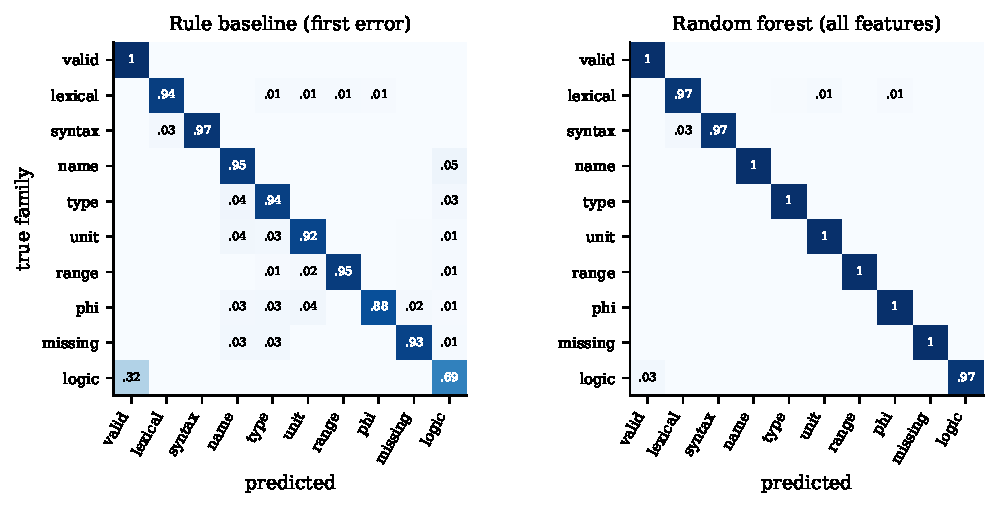
\includegraphics[width=0.8\textwidth]{figs/confusion.pdf}
\caption{Row-normalised confusion matrices on the test set. Left: ``first error'' rule. Right: random forest.}
\label{fig:confusion}
\end{figure}

Figure~\ref{fig:confusion} shows where the rules fall short.

\begin{itemize}
    \item \textbf{Faults the compiler cannot see.} 63 of the 200 \emph{logic} test programs are reported clean by both
    rules, so their logic recall is only \RuleLogicRecall\%. These are inverted rules and mismatched alert texts in
    programs that are otherwise well formed and unit-correct. The forest gets \RFLogicRecall\% recall on logic, using the
    pattern features.
    \item \textbf{Cascades hide lexical root causes.} ``Most severe'' is perfect on the six semantic families, which is
    expected since it is the labelling rule. It fails on lexical programs: an unterminated string swallows the rest of its
    line, the parser then reports syntax errors, and the rule picks the symptom (73 of 200 programs).
    \item \textbf{The first diagnostic is often not the root cause.} On two-fault programs ``first error'' is right only
    \RuleFirstDouble\% of the time, against 96.2\% on single-fault ones. The forest gets \RFDouble\% of two-fault programs.
    \item \textbf{What is left.} The forest makes 17 mistakes: six soft logic faults taken for valid, five syntax
    programs taken for lexical, and six lexical programs put in a semantic family. The lexical/syntax confusion is the
    same cascade problem and is not fully solved.
\end{itemize}

So machine learning does not beat a well-built rule set on the faults the rules were written for; there the analyser
is already at 100\%. The gain is in the cases the rules miss or mislabel. Also, the test programs come from the same
generator as the training programs, so 99\% is an in-distribution number (see Section~\ref{sec:limits}). The forest's most important
feature by far is \code{worst\_family\_rank} (importance 0.142), followed by counts of individual diagnostic codes such as
\code{DOM002} and \code{DOM001}. The learned classifier is mostly a learned post-processor of the compiler's output,
which is what the design intended.

\subsection{Which Feature Groups Matter (E2)}

\begin{table}[!htbp]
\centering
\caption{Random-forest test macro-F1 by feature view and training programs per class (mean of five draws).}
\label{tab:learning}
\small
\begin{tabular}{lrrrrrrr}
\toprule
\textbf{Feature view} & \textbf{5} & \textbf{10} & \textbf{25} & \textbf{50} & \textbf{100} & \textbf{200} & \textbf{800}\\
\midrule
token+AST & 0.142 & 0.187 & 0.258 & 0.326 & 0.373 & 0.398 & 0.436\\
diagnostics & 0.918 & 0.937 & 0.942 & 0.950 & 0.960 & 0.963 & 0.967\\
diagnostics+patterns & 0.918 & 0.946 & 0.970 & 0.979 & 0.988 & 0.991 & 0.994\\
all features & 0.884 & 0.926 & 0.950 & 0.969 & 0.983 & 0.988 & 0.991\\\bottomrule
\end{tabular}

\end{table}

Table~\ref{tab:learning} gives three results. Token and tree statistics alone are weak: 0.14 macro-F1 with five programs
per class and 0.44 with 800. A forest cannot rebuild from raw counts what a unit checker or a taint analysis computes,
which is the clearest argument in the data for putting a real compiler under the learner. Diagnostics alone level off
at 0.967 because they cannot see soft logic faults, and the six pattern features take that to 0.994. Finally, using all
features is slightly worse than diagnostics plus patterns at every size (0.884 against 0.918 at five per class), since
the 55 token and tree dimensions mostly add noise. We still kept the full vector for the GAN experiments because it is
what the deployed classifier uses. With five labelled programs per class the forest is at 0.88, and the next question
is whether synthetic records can close the gap to 0.99.

% ============================================================
% RESULTS (part B): GAN augmentation and GAN anomaly detection
% ============================================================
\subsection{Augmentation under Scarcity: Does the GAN Help? (E3)}

This is the experiment the GAN was there for: with only a handful of real faulty programs per class, do synthetic
vectors help? Figure~\ref{fig:augment} and Table~\ref{tab:augrf} give test macro-F1 for the seven regimes over ten seeds.

\begin{figure}[!htbp]
\centering
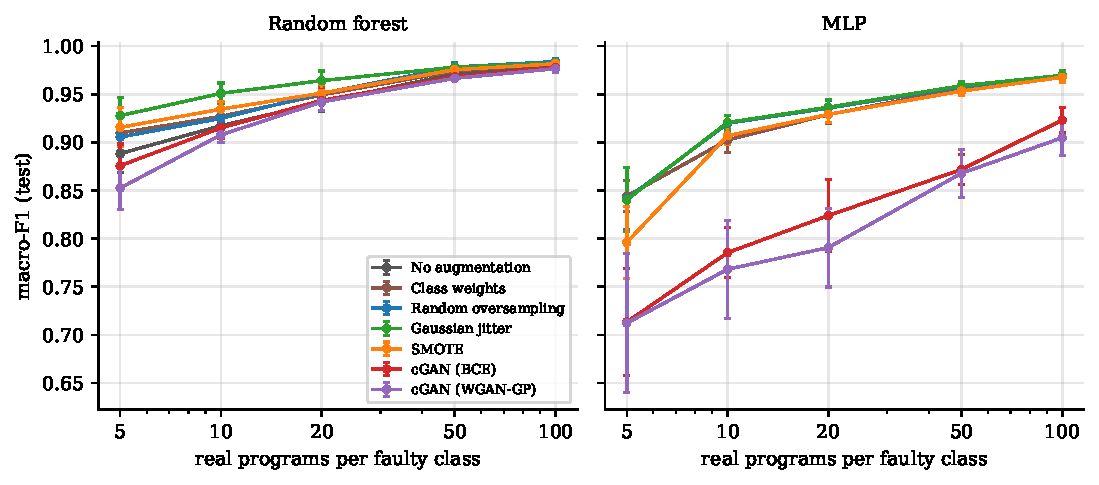
\includegraphics[width=0.9\textwidth]{figs/augment.pdf}
\caption{Test macro-F1 against real training programs per faulty class (mean $\pm$ s.d. over ten seeds). Left: random
forest. Right: MLP.}
\label{fig:augment}
\end{figure}

\begin{table}[!htbp]
\centering
\caption{Random forest: test macro-F1 (mean $\pm$ s.d., ten seeds) by real programs per faulty class. Bold is the best
mean per column.}
\label{tab:augrf}
\small
\resizebox{\textwidth}{!}{\begin{tabular}{lccccc}
\toprule
\textbf{Method} & \textbf{5} & \textbf{10} & \textbf{20} & \textbf{50} & \textbf{100}\\
\midrule
No augmentation & 0.888\,$\pm$\,0.020 & 0.917\,$\pm$\,0.009 & 0.942\,$\pm$\,0.009 & 0.971\,$\pm$\,0.003 & 0.979\,$\pm$\,0.003\\
Class weights & 0.910\,$\pm$\,0.018 & 0.927\,$\pm$\,0.008 & 0.949\,$\pm$\,0.008 & 0.974\,$\pm$\,0.004 & 0.982\,$\pm$\,0.003\\
Random oversampling & 0.906\,$\pm$\,0.020 & 0.925\,$\pm$\,0.010 & 0.951\,$\pm$\,0.009 & \textbf{0.978\,$\pm$\,0.004} & \textbf{0.984\,$\pm$\,0.003}\\
Gaussian jitter & \textbf{0.928\,$\pm$\,0.019} & \textbf{0.951\,$\pm$\,0.011} & \textbf{0.964\,$\pm$\,0.010} & 0.978\,$\pm$\,0.002 & 0.982\,$\pm$\,0.003\\
SMOTE & 0.916\,$\pm$\,0.020 & 0.935\,$\pm$\,0.008 & 0.951\,$\pm$\,0.009 & 0.975\,$\pm$\,0.005 & 0.982\,$\pm$\,0.003\\
cGAN (BCE) & 0.876\,$\pm$\,0.023 & 0.915\,$\pm$\,0.011 & 0.944\,$\pm$\,0.011 & 0.968\,$\pm$\,0.003 & 0.978\,$\pm$\,0.003\\
cGAN (WGAN-GP) & 0.853\,$\pm$\,0.022 & 0.908\,$\pm$\,0.008 & 0.942\,$\pm$\,0.009 & 0.967\,$\pm$\,0.001 & 0.977\,$\pm$\,0.004\\\bottomrule
\end{tabular}
}
\end{table}

\paragraph{The short answer is no.} With the random forest the GAN is never the best method and is usually within noise
of doing nothing: 0.944 against 0.942 at 20 programs per class, and worse at five (0.876 for BCE and 0.853 for WGAN-GP,
against 0.888). The cheap methods do better. Gaussian jitter is best at every size up to 20 (0.928 against 0.888 at
five), and SMOTE, oversampling and class weights give smaller gains. By 100 programs everything is within a point. For
the MLP it is worse: GAN vectors cost 5 to 13 points of macro-F1, most at the smallest sizes (0.713 against 0.844 at
five), probably because an MLP tries to fit every synthetic point where a forest can ignore some. Paired $t$-tests over
the seeds show the GAN's difference from no augmentation is either indistinguishable from zero or slightly negative, and
its difference from jitter and SMOTE is negative at every size.

Almost all of the gain from augmentation comes from one class. Most classes are near their ceiling without help, but
\emph{logic}, which has to be recognised largely from the six pattern features, goes from F1 0.52 with no augmentation to
0.79 with jitter at five programs, while the BCE GAN gives 0.47. Augmentation here mostly works as a regulariser for the
one hard class.

\paragraph{Why the GAN fails.} For one seed at 20 programs per class we inspected the synthetic vectors
(Table~\ref{tab:fidelity}). \emph{Label validity} is the share that an oracle forest trained on the full pool assigns to
the requested class. \emph{NN distance} is the mean standardised distance to the nearest real training vector of that
class; held-out real programs sit at \HeldoutNN{} for comparison.

\begin{table}[!htbp]
\centering
\caption{Fidelity of synthetic vectors (seed 0, 20 real programs per faulty class). Resampling methods score high on
label validity by construction, since their points sit on or next to real vectors.}
\label{tab:fidelity}
\small
\begin{tabular}{lrrr}
\toprule
\textbf{Generator} & \textbf{Label validity} & \textbf{NN distance} & \textbf{Exact copies (\%)}\\
\midrule
Random oversampling & 1.000 & 0.00 & 100.0\\
Gaussian jitter & 1.000 & 0.84 & 0.0\\
SMOTE & 1.000 & 3.01 & 0.0\\
cGAN (BCE) & 0.037 & 11.30 & 0.0\\
cGAN (WGAN-GP) & 0.043 & 10.80 & 0.0\\\bottomrule
\end{tabular}

\end{table}

Only 4\% of GAN vectors are recognised as the requested class, below the 10\% you would get by guessing, and they lie
further from the training data than new real programs do. The generator did not learn the class structure. One likely
cause was that mini-batches were dominated by the 400 valid programs, so we reran with class-balanced batches (five
seeds). Label validity rose to 11 to 13\%, about chance, and macro-F1 did not improve. The rest of the explanation is the
obvious one: 20 examples per class in a 101-dimensional space of counts is too little for a small unregularised GAN, and
a continuous generator blurs features with discrete, tightly linked meaning (a count of exactly one for exactly one
code). This is a limit of our setup, not a verdict on GANs; we did not try tabular models such as CTGAN~\cite{xu2019} or
any tuning. In this setting, simple resampling is the better way to handle rare error classes.

\subsection{GAN-Based Anomaly Detection (E4)}

The second use of a GAN is to find faulty programs when no faulty examples exist at all. Table~\ref{tab:anomaly} gives
the AUROC of each detector, trained on valid programs only, for separating valid test programs from each fault family.

\begin{table}[!htbp]
\centering
\caption{AUROC of valid-versus-faulty detection by fault family.}
\label{tab:anomaly}
\small
\resizebox{\textwidth}{!}{\begin{tabular}{lrrrrr}
\toprule
\textbf{Fault family} & \textbf{Isolation Forest} & \textbf{One-class SVM} & \textbf{GAN discriminator (BCE)} & \textbf{GAN critic (WGAN-GP)} & \textbf{Compiler error flag}\\
\midrule
lexical & 0.471 & 0.905 & 1.000 & 0.388 & 1.000\\
syntax & 0.465 & 0.901 & 1.000 & 0.310 & 1.000\\
name & 0.475 & 0.806 & 1.000 & 0.381 & 1.000\\
type & 0.498 & 0.839 & 1.000 & 0.392 & 1.000\\
unit & 0.454 & 0.834 & 1.000 & 0.360 & 1.000\\
range & 0.451 & 0.867 & 1.000 & 0.433 & 1.000\\
phi & 0.498 & 0.865 & 1.000 & 0.265 & 1.000\\
missing & 0.495 & 0.885 & 1.000 & 0.325 & 1.000\\
logic & 0.452 & 0.715 & 0.981 & 0.487 & 0.843\\
all faults & 0.473 & 0.846 & 0.998 & 0.371 & 0.982\\\bottomrule
\end{tabular}
}
\end{table}

\begin{itemize}
    \item \textbf{The BCE discriminator scores 0.998 overall, but most of that is easy.} 49 of the 101 features,
    including all 40 diagnostic ones, are constant on valid programs because a valid program has no diagnostics. The
    compiler's own ``at least one error'' flag gets 1.000 on every family except logic.
    \item \textbf{The column that matters is logic.} There the compiler flag drops to 0.843, the one-class SVM gets 0.715,
    and the BCE discriminator 0.981. Over five retraining seeds it stays between 0.97 and 0.99. Without the pattern
    features it falls to 0.83 to 0.87, and the pattern features alone give 0.60 to 0.69, so the discriminator wins by
    combining the two signals.
    \item \textbf{Isolation Forest sits at chance (0.47)}, even after removing the constant features: among the features
    that do vary, faulty programs look like valid ones.
    \item \textbf{The WGAN-GP critic fails at 0.37}, below chance. A critic learns to separate real from generated
    samples, not to model density, and it extrapolates badly off the data. Flipping the sign would give about 0.63, but we
    report the score as defined before seeing the result.
\end{itemize}

So a discriminator trained only on valid programs is a usable unsupervised detector for the one family the compiler
misses. It is not better than the compiler on the families the compiler handles.

% ============================================================
% RESULTS (part C): compiler performance, case studies, validity
% ============================================================
\subsection{Compiler Performance and Worked Examples (E5)}

For valid programs from 46 to 12{,}016 lines, a linear fit of total compile time against size gives \MsPerKloc{} ms per
thousand lines ($R^2=\ScaleRSq$), so a 40-line corpus program compiles in a few milliseconds. The log-log slope at large
sizes is \ScaleSlope, a little worse than linear. The cause is the semantic phase: it takes about a quarter of the time up
to 800 lines but 53\% at 12{,}000 lines, because every \code{if} copies the flow state, which grows with the number of
top-level declarations. Sharing those sets between branches would fix it, and at the size of real clinical scripts it
does not matter.

Across 300 generated programs the optimiser removed on average \OptMean\% of the three-address instructions (maximum
\OptMax\%), and the original and optimised code produced identical output on ten random inputs every time
(\OptMismatch{} mismatches in \OptPrograms{} programs). Generated programs have little redundancy, so the gain is modest.
On a demo program with constant arithmetic, the optimiser folds the constants, shares a repeated product
\code{per\_kg * weight} and deletes a dead branch, going from 18 instructions to 11. It still leaves a jump to the next
label (there is no peephole pass) and does not propagate across labels; neither affects correctness.

The command-line tool prints the compiler's diagnostics followed by the classifier's root-cause estimate.
Listing~\ref{lst:phi} shows a program with four faults: PHI concatenated into output, a temperature threshold missing
its decimal point (caught by both the range and the plausibility check), and a dose added to a weight. The classifier
ranks \emph{phi} first, which matches the root-cause priority.

\begin{lstlisting}[language={},numbers=none,basicstyle=\ttfamily\scriptsize,caption={Output of \texttt{medcheck.py examples/phi\_leak.med}.},label={lst:phi}]
== examples/phi_leak.med: 100 tokens, 4 error(s), 0 warning(s)
  12:19: error DOM002: protected health information reaches print() without anonymize()
  13:10: error DOM001: comparison against 380, outside the declared range [30, 43] of 'temp'
  13:12: error DOM001: value 380 degC is outside the plausible range [20.0, 45.0] degC
  16:12: error SEM005: unit mismatch: [mg] + [kg]
== learned root-cause estimate: phi 0.80, range 0.11, lexical 0.06
\end{lstlisting}

The more interesting case is a program the compiler has nothing to say about. In the example file
\texttt{inverted\_rule.med} the fever rule reads \code{if (temp < 38.0 degC)}. It compiles without a single
diagnostic, and the forest still puts it in \emph{logic} with probability 0.77 (valid 0.20). The tool prints a note
that the front end found no error but the classifier suspects a clinical-logic fault. It is worded as a suspicion
because it is an estimate from a model trained on synthetic faults, not a proof.

\subsection{Threats to Validity}
\label{sec:limits}

\begin{itemize}
    \item \textbf{Synthetic, in-distribution test.} Training and test programs come from the same generator and the same
    operators. The near-perfect accuracy shows how well the classifier learned this generator's faults. It says little
    about hand-written MedScript and nothing about real clinical code.
    \item \textbf{Labels come from the injection.} We checked that each fault shows up in the compiler, not that a human
    would call it the root cause. The ``most severe'' baseline is the labelling rule applied to diagnostics, so its 100\%
    on semantic families is partly circular.
    \item \textbf{Hand-written vocabulary.} The pattern features depend on a list of alert words, and a program that names
    its alerts differently would get past them.
    \item \textbf{No tuning.} Hyper-parameters were fixed in advance and never tuned, so a better-tuned GAN might do better.
    The scarcity range in E3 was widened after a pilot run on a separate, smaller corpus.
\end{itemize}

% ============================================================
% CONCLUSION
% ============================================================
\section{Conclusion and Future Work}

We set out to build a compiler for medical data-processing programs that understands the domain, plus a learned
component that classifies errors and uses a GAN to cope with scarce labelled data. The first two parts worked. The third
did not.

The MedScript compiler has the usual phases (scanner, recursive-descent parser with error recovery, semantic analyser,
three-address code, optimiser) and a semantic phase extended with checks that matter in healthcare: units through
dimension vectors, physiological plausibility through intervals, taint tracking of patient identifiers, flow-sensitive
handling of optional values, definite assignment and division by zero. All 38 unit tests pass, the optimiser preserved
behaviour on all 300 tested programs, and compilation runs at about \MsPerKloc{} ms per thousand lines.

A random forest over 101 compiler-derived features reached \RFAcc\% accuracy on 2{,}000 held-out programs, against
\RuleFirstAcc\% and \RulePrioAcc\% for the two rule baselines. The gain comes from faults with no diagnostic (inverted
clinical rules) and from programs where cascades or a second fault make the first message misleading. Surface features
alone reach only 0.44 macro-F1, so the learner is only as useful as the compiler underneath it.

The GAN result is negative, and we think that is worth reporting. With 5 to 100 real programs per faulty class,
conditional GANs gave nothing over no augmentation for a random forest and a clear loss for an MLP, while Gaussian jitter
and SMOTE gained up to four points. Only about 4\% of GAN samples looked like the class they were meant to be. A GAN
discriminator trained on valid programs did turn out to be a good detector of the faults the compiler misses (AUROC about
0.98), which is a narrower use than the one we started with. All of these numbers come from a synthetic corpus and should
be read that way.

\paragraph{Future work.} The most important next step is real data: hand-written MedScript from people who never saw the
generator, and a port of the unit, PHI and missing-value checks to Python or R through an AST-based analyser. On the
learning side, tabular generators such as CTGAN with proper handling of discrete features are worth trying, as is
generating programs instead of feature vectors so that synthetic examples can be compiled and checked. Other directions
are locating the line of a soft fault with a graph model over the syntax tree, implicit unit conversion and
inter-procedural taint, a stronger back end targeting LLVM IR, and a user study on whether the root-cause estimate
actually helps developers find faults faster.

% ============================================================
% REFERENCES
% ============================================================
\small
\begin{thebibliography}{99}
\setlength{\itemsep}{1pt}

\bibitem{aho2006}
A. V. Aho, M. S. Lam, R. Sethi, and J. D. Ullman,
\textit{Compilers: Principles, Techniques, and Tools},
2nd ed., Pearson/Addison-Wesley, 2006.

\bibitem{cooper2007}
K. D. Cooper and L. Torczon,
\textit{Engineering a Compiler},
2nd ed., Morgan Kaufmann, 2011.

\bibitem{grune2008}
D. Grune and C. J. H. Jacobs,
\textit{Parsing Techniques: A Practical Guide},
2nd ed., Springer, 2008.

\bibitem{burke1987}
M. G. Burke and G. A. Fisher,
``A practical method for LR and LL syntactic error diagnosis and recovery,''
\textit{ACM Transactions on Programming Languages and Systems}, vol. 9, no. 2, pp. 164--197, 1987.

\bibitem{nielson1999}
F. Nielson, H. R. Nielson, and C. Hankin,
\textit{Principles of Program Analysis},
Springer, 1999.

\bibitem{kennedy1994}
A. Kennedy,
``Dimension types,''
in \textit{Proc. European Symposium on Programming (ESOP)}, LNCS vol. 788, Springer, 1994, pp. 348--362.

\bibitem{enck2010}
W. Enck et al.,
``TaintDroid: An information-flow tracking system for realtime privacy monitoring on smartphones,''
in \textit{Proc. 9th USENIX Symposium on Operating Systems Design and Implementation (OSDI)}, 2010, pp. 393--407.

\bibitem{hipaa}
U.S. Department of Health and Human Services,
``Standards for privacy of individually identifiable health information,''
45 CFR Parts 160 and 164 (HIPAA Privacy Rule).

\bibitem{leveson1993}
N. G. Leveson and C. S. Turner,
``An investigation of the Therac-25 accidents,''
\textit{IEEE Computer}, vol. 26, no. 7, pp. 18--41, 1993.

\bibitem{mco1999}
Mars Climate Orbiter Mishap Investigation Board,
\textit{Phase I Report},
NASA, November 1999.

\bibitem{allamanis2018}
M. Allamanis, E. T. Barr, P. Devanbu, and C. Sutton,
``A survey of machine learning for big code and naturalness,''
\textit{ACM Computing Surveys}, vol. 51, no. 4, article 81, 2018.

\bibitem{gupta2017}
R. Gupta, S. Pal, A. Kanade, and S. Shevade,
``DeepFix: Fixing common C language errors by deep learning,''
in \textit{Proc. AAAI Conference on Artificial Intelligence}, 2017, pp. 1345--1351.

\bibitem{pradel2018}
M. Pradel and K. Sen,
``DeepBugs: A learning approach to name-based bug detection,''
\textit{Proc. ACM on Programming Languages}, vol. 2, no. OOPSLA, article 147, 2018.

\bibitem{goodfellow2014}
I. Goodfellow et al.,
``Generative adversarial nets,''
in \textit{Advances in Neural Information Processing Systems 27}, 2014.

\bibitem{mirza2014}
M. Mirza and S. Osindero,
``Conditional generative adversarial nets,''
arXiv:1411.1784, 2014.

\bibitem{salimans2016}
T. Salimans, I. Goodfellow, W. Zaremba, V. Cheung, A. Radford, and X. Chen,
``Improved techniques for training GANs,''
in \textit{Advances in Neural Information Processing Systems 29}, 2016.

\bibitem{arjovsky2017}
M. Arjovsky, S. Chintala, and L. Bottou,
``Wasserstein generative adversarial networks,''
in \textit{Proc. 34th International Conference on Machine Learning (ICML)}, PMLR vol. 70, 2017, pp. 214--223.

\bibitem{gulrajani2017}
I. Gulrajani, F. Ahmed, M. Arjovsky, V. Dumoulin, and A. Courville,
``Improved training of Wasserstein GANs,''
in \textit{Advances in Neural Information Processing Systems 30}, 2017.

\bibitem{choi2017}
E. Choi, S. Biswal, B. Malin, J. Duke, W. F. Stewart, and J. Sun,
``Generating multi-label discrete patient records using generative adversarial networks,''
in \textit{Proc. Machine Learning for Healthcare Conference (MLHC)}, PMLR vol. 68, 2017, pp. 286--305.

\bibitem{xu2019}
L. Xu, M. Skoularidou, A. Cuesta-Infante, and K. Veeramachaneni,
``Modeling tabular data using conditional GAN,''
in \textit{Advances in Neural Information Processing Systems 32}, 2019.

\bibitem{chawla2002}
N. V. Chawla, K. W. Bowyer, L. O. Hall, and W. P. Kegelmeyer,
``SMOTE: Synthetic minority over-sampling technique,''
\textit{Journal of Artificial Intelligence Research}, vol. 16, pp. 321--357, 2002.

\bibitem{schlegl2017}
T. Schlegl, P. Seeb\"ock, S. M. Waldstein, U. Schmidt-Erfurth, and G. Langs,
``Unsupervised anomaly detection with generative adversarial networks to guide marker discovery,''
in \textit{Proc. Information Processing in Medical Imaging (IPMI)}, LNCS vol. 10265, Springer, 2017, pp. 146--157.

\bibitem{liu2008}
F. T. Liu, K. M. Ting, and Z.-H. Zhou,
``Isolation forest,''
in \textit{Proc. IEEE International Conference on Data Mining (ICDM)}, 2008, pp. 413--422.

\bibitem{scholkopf2001}
B. Sch\"olkopf, J. C. Platt, J. Shawe-Taylor, A. J. Smola, and R. C. Williamson,
``Estimating the support of a high-dimensional distribution,''
\textit{Neural Computation}, vol. 13, no. 7, pp. 1443--1471, 2001.

\bibitem{breiman2001}
L. Breiman,
``Random forests,''
\textit{Machine Learning}, vol. 45, no. 1, pp. 5--32, 2001.

\bibitem{pedregosa2011}
F. Pedregosa et al.,
``Scikit-learn: Machine learning in Python,''
\textit{Journal of Machine Learning Research}, vol. 12, pp. 2825--2830, 2011.

\bibitem{paszke2019}
A. Paszke et al.,
``PyTorch: An imperative style, high-performance deep learning library,''
in \textit{Advances in Neural Information Processing Systems 32}, 2019.

\bibitem{kingma2015}
D. P. Kingma and J. Ba,
``Adam: A method for stochastic optimization,''
in \textit{Proc. International Conference on Learning Representations (ICLR)}, 2015.

\bibitem{sokolova2009}
M. Sokolova and G. Lapalme,
``A systematic analysis of performance measures for classification tasks,''
\textit{Information Processing \& Management}, vol. 45, no. 4, pp. 427--437, 2009.

\bibitem{fawcett2006}
T. Fawcett,
``An introduction to ROC analysis,''
\textit{Pattern Recognition Letters}, vol. 27, no. 8, pp. 861--874, 2006.

\bibitem{muchnick1997}
S. S. Muchnick,
\textit{Advanced Compiler Design and Implementation},
Morgan Kaufmann, 1997.

\end{thebibliography}

\end{document}
